\chapter{Multi-Agent Simulator of Neighborhoods}
\label{Chapter.four}

MASON~\cite{MASON, MASON2005, MASONMANUAL2011} is an open source, domain independent and multiagent simulator which supports various agents in a single system. It is an easily extensible, fast, flexible and discrete-event simulator~\cite{MASON2005}. Simulation core and visualization libraries of MASON are completely written in Java. Unlike in other simulators any experienced Java user can easily add or modify some features which are not domain-specific. Most of the simulation toolkits are designed for small tasks. The main advantage in choosing MASON is that it is meant for huge and complex multiagent simulation tasks involving several simulation runs. It has a good simulation speed and also documentation is sufficient enough when compared to the other toolkits. There is a vast amount of research on multiagent simulations as they are currently used in applications such as robotics, security and defense systems, and unmanned aerial and underwater vehicles. Using MASON we can easily create multiagent simulation models and can run several of them in parallel on back-end machines. MASON's properties, architecture and architectural layers are discussed in the following sections.

\section{Architecture}

MASON is comprised of two parts, model and visualization~\cite{MASONMANUAL2011}. Both of them can be in either 2D or 3D. Model and visualization are independent until and unless we choose to have model objects display themselves. It is also possible to run a model without visualization. It can support up to a million agents when we are not using any visualization. Running a model with or without visualization can be controlled by the designer. MASON models can be entirely serializable to disk. This means that the files can be checkpointed and can be resumed later. MASON models are completely encapsulated; We can run two models independently in the same process without interrupting each other. In order to overcome Java's reputation of being slow, some Sun (subsidiary of Oracle corporation) classes are replaced by MASON equivalents which perform more accurately. One such class is MASON's random number generator which is supposedly high in quality when compared to the one in Java. Usage of Java language in modeling makes the model more flexible to run in heterogeneous computer environments. MASON models are also duplicable, that is, simulation results on different machines will remain the same when the simulation is carried out using the same parameters. 

When choosing MASON as a simulation toolkit for creating models, we need to consider the following aspects :

\begin{enumerate}
\item MASON is not intended to achieve parallelization of an individual simulation. It cannot be used when there is a need to distribute a single simulation among multiple processors.   
\item MASON core is meant to be simple, and hence it does not provide any built-in features specific to robotics simulators or other social agents.
\item MASON toolkit is not designed for creating memory efficient models. It can only be moderately memory efficient. 
\end{enumerate}

Apart from the above mentioned limitations, MASON is good in certain aspects such as model detachment from visualization, check-pointing, speed,  portability and strong visualizations. These features are commonly considered as assets among the simulation community.

Java language is chosen to build MASON toolkit in order to take the advantage of its strict math and type definitions, portability and object serialization. These properties of Java will help MASON models to achieve duplicability and also to checkpoint the simulations.

MASON toolkit has three layers: utility layer, the model layer and the visualization layer. Firstly, the utility layer has classes that are used for many purposes. These classes include data structures, a random-number generator, which are more powerful than those available in Java distribution, movie and snapshot generating facilities and various Graphical User Interface (GUI) widgets. Secondly, the model layer consists of classes such as schedule utilities, a discrete event schedule, and a collection of fields that include objects and combine them with locations. This code alone will allow the developer to create basic simulations which can be run from the command line. Finally, the visualization layer enables GUI based visualization and manipulation of the created model. Model and visualization layers are  further explained in Section~\ref{Section.two} and Section~\ref{Section.three} respectively. The pictorial representation of these two layers and their classes are shown in Fig.\ref{fig:4.1}.

\section{Model Layer}
\label{Section.two}

Model layer in MASON does not have any dependencies on Visualization layer and can be easily detached from it. MASON's model is enclosed within an instance of user-defined subclass of a class called \texttt{SimState}. This instance consists of a \texttt{MersenneTwister} random number generator, a discrete event \texttt{Schedule} and zero or more fields~\cite{MASON2005}.

\vspace{15mm}
\begin{figure}[H]
\flushleft
\includegraphics[height=7.2in, width=4.6in]{Mason_layers.eps}
\caption[Simplified UML diagram of basic classes]{Simplified UML diagram which consists of basic classes present in model and visualization layers. Labels in parenthesis indicate the sets from which several classes are available~\cite{MASON2005}.}
\label{fig:4.1}
\end{figure} 


\vspace{10mm}
\noindent\textbf{Agents and the Schedule}
\vspace{5mm}

\noindent In the context of MASON, agents are computational units that can be scheduled to implement a certain action and to manipulate the environment. MASON directly schedules an agent to be \textit{stepped} (or called) at some particular time rather than scheduling other events to be sent to an agent. Agents created in MASON implements the \texttt{Steppable} interface as illustrated in Fig.\ref{fig:4.1}. Anonymous wrapper class allows agents to schedule several times to  accomplish different functions. MASON is capable of scheduling steppable objects at any point of time in the near future. Additionally, a schedule can be split into various \textit{orderings} which subdivide the given time step: at any given time the scheduled agents which are in earlier ordering will be stepped prior to those of scheduled agents in the later ordering. MASON has several \texttt{Steppable} wrappers of which some can group agents together, perform them in parallel on separate threads and iterate them. Agents can be scheduled to run asyncronously with the schedule in their own thread. This thread can loop indefinitely, run continously until completion or run till the \texttt{Schedule} arrives at the next time step.

\vspace{0.5cm} 
\noindent\textbf{Fields}
\vspace{5mm}

\noindent MASON's fields associate arbitrary values or objects to locations in some abstract space. Some of these fields are a bit more than wrappers for simple 2D/3D arrays, whereas other fields cater to sparse relationships. An object can be present in different fields at the same time and the same object may also exist multiple times in some fields. The usage of these fields in an application can be optional. There is a possibility for a user to design and add his or her own fields. MASON is providing fields for the following~\cite{MASON2005}: 

\begin{enumerate}
 \item The edges of Networks (graphs) which may be either directed or undirected and optionally weighted or labeled.
 \item 2D and 3D bounded arrays of integers, objects or doubles, which can be toroidal or bounded as per user requirements, and can also be with triangular, hexagonal or square layouts.
 \item 2D and 3D sparsely populated object grids. These grids can be toroidal, bounded or unbounded. These may also be with triangular, hexagonal or square layouts.
 \item 2D and 3D sparse continuous space, which can be toroidal, bounded or unbounded.
\end{enumerate}
\vspace{5mm}

 When a model is run without any visualization, MASON has a primary top level simulation loop. MASON initiates either by creating a entirely new \texttt{SimState} or by loading it from Java serialized checkpoint file. MASON then starts the successive loop. Firstly, it checks for the remaining agents in the \texttt{Schedule} to step. If there are no agents, or if the maximum time limit in the \texttt{Schedule} has been exceeded, MASON quits the loop, completes the \texttt{SimState} and halts. Secondly, the \texttt{Schedule} increases its time to be equivalent to the minimum time step for the agents to \texttt{Schedule} and then steps all agents whose \texttt{Schedule} starts at that time step. If checkpoint of the model is needed, that can be done at this point of time. Check-pointing can be done in three steps as stated below.
 
\begin{enumerate}
 \item A request is sent to all asynchronous agents to pause their threads, 
 \item Entire model checkpoint is written out.
 \item All threads related to asynchronous agents are resumed, and the loop proceeds further. 
\end{enumerate}
\vspace{5mm}

Agents can access the \texttt{SimState} to full extent and can manipulate its \texttt{Schedule}, random number generator, and fields. MASON has few restrictions on the actions of the agents and it does not provide any simple protocols for designing an agent.

\section{Visualization Layer}
\label{Section.three}

\texttt{GUIState} is wrapped around \texttt{SimState} and acts as a gatekeeper. Visualization layer objects can examine the objects of Model layer only after the approval from \texttt{GUIState}. When running a model with GUI, \texttt{GUIState} class is responsible for attaching or detaching the visualization with \texttt{SimState} and also to checkpoint the \texttt{SimState} to or from disk. As some of the objects in the visualization group requires to be scheduled (particularly, windows must be refreshed to take the effect of new changes in the model), these elements can ``schedule'' by themselves along with the \texttt{GUIState} to be restored when the fundamental \texttt{Schedule} is pulsed but not scheduled on the actual \texttt{Schedule} itself. All of this supports the visualization layer being able to separate from the actual model.

Besides the \texttt{SimState}, \texttt{GUIState} can also manage zero or more displays, GUI windows which are capable of providing both 2D and 3D views of primary fields. Displays act upon by taking hold of zero or more \textit{field portrayals}, correlating each one with a distinct field in a model. Every field portrayal is bound to draw a field on the screen and to act in response to user requests to inspect the fields features. \textit{Field portrayals} accomplish by correlating \textit{simple portrayals} with specific objects or values which are stored in the fields. Simple portrayals may also, on demand, call inspectors of fundamental objects. Inspectors are nothing but GUI panels which grant user to modify and inspect parameters of objects. User can create his/her own inspectors or can access the available basic ones. 

The GUI window is a top level controller for the \texttt{GUIState}, which is commonly the given console. \texttt{Consoles} fundamental functionality is to authorize user to play, pause, stop , step the schedule. 

Apart from the above mentioned basic functionality the console also provides the following GUI functionalities: 
\begin{enumerate}
\item Allows user to save and load models which are checkpointed 
\item Hides and shows the displays as per user requirements
\item Helps user in viewing the inspectors 
\item Permits user to load additional simulations (each of which has its own individual \texttt{SimStates}, \texttt{GUIStates} and \texttt{Consoles}).
\end{enumerate}
\vspace{5mm}

To run a model without visualization is less complex when compared to a model with visualization, not only because of including display but based on the following explanation. A fundamental model runs on its very own thread which is independent from the GUI's main thread and both threads need to access the model data. For this reason, GUI thread and the model thread enters into synchronization procedure which assures that only one of these threads have access model data at any given point of time. The whole process is further explained in next few sentences. When \texttt{GUIState} is built, it in turn constructs a \texttt{Console}, several displays, and the fundamental \texttt{SimState}. In the \texttt{Console} a user can initiate the simulation by pressing ``play`` which allows the \texttt{Console} to start the \texttt{SimState} and then creates the model thread. The model thread will then enter into the loop and then quits the loop either when the \texttt{Console} asks to shut down or if there are no more scheduled agents. In the loop which was mentioned in the above statement, the \texttt{GUIState} completes some pre-scheduled items, then the schedule progresses to the minimum time step required for the agents to start scheduling and then steps all the agents at that point of time. After this, post-scheduled items are completed and then the model thread suspends and give the GUI thread access to model. While model thread is in waiting state, the GUI thread completes redrawing the displays, checks for the users requests for model inspection if any, and checkponts the model. When a user press ''Stop`` from the \texttt{Console}, the thread is requested for a shut down and the \texttt{Console} completes the \texttt{SimState}. When user closes the \texttt{Console}, the \texttt{SimState}, displays and  \texttt{GUIStates} are destroyed.


\subsection{Dependencies of MASON}
The following are required, in order to keep MASON simulation toolkit up and running: JDK (higher version than 1.3), JFreeChat, JCommon, JMF, iText and Java3D (to run 3D models).

